%% thesis.tex 2014/04/11
%
% Based on sample files of unknown authorship.
%
% The Current Maintainer of this work is Paul Vojta.

\documentclass{ucbthesis}
\usepackage{biblatex}
\usepackage{rotating} % provides sidewaystable and sidewaysfigure
\usepackage{textcomp} % degrees symbol
\usepackage{siunitx} % units
\usepackage{amsmath,amssymb,amsfonts,hyperref,lineno,microtype,setspace,multicol,textcomp, marvosym, algorithm,algpseudocode, algorithmicx, wrapfig, mathtools}

% hyperref colors
%\hypersetup{
  %colorlinks,
  %citecolor=violet,
  %linkcolor=black,
  %urlcolor=blue}
\hypersetup{colorlinks=true, citecolor=green, linkcolor=black, urlcolor=blue}


% To compile this file, run "latex thesis", then "biber thesis"
% (or "bibtex thesis", if the output from latex asks for that instead),
% and then "latex thesis" (without the quotes in each case).

% Double spacing, if you want it.  Do not use for the final copy.
% \def\dsp{\def\baselinestretch{2.0}\large\normalsize}
% \dsp

% If the Grad. Division insists that the first paragraph of a section
% be indented (like the others), then include this line:
% \usepackage{indentfirst}

\addtolength{\abovecaptionskip}{\baselineskip}

\newtheorem{theorem}{Jibberish}

\bibliography{aroma_7}

\hyphenation{mar-gin-al-ia}
\hyphenation{bra-va-do}

\begin{document}

% Declarations for Front Matter

\title{Structural Insights for Molecular Design of Conjugated Molecule and Polymers}
\author{Brandon Wood}
\degreesemester{Summer}
\degreeyear{2019}
\degree{Doctor of Philosophy}
\chair{Associate Professor Kristin Persson}
\othermembers{The Aldo DeBenedictis Distinguished Professor Phillip Geissler\\
Professor Daryl Chrzan}


% For a co-chair who is subordinate to the \chair listed above
% \cochair{Professor Benedict Francis Pope}
% For two co-chairs of equal standing (do not use \chair with this one)
% \cochairs{Professor Richard Francis Sony}{Professor Benedict Francis Pope}
\numberofmembers{3}
% Previous degrees are no longer to be listed on the title page.
% \prevdegrees{B.A. (University of Northern South Dakota at Hoople) 1978 \\
%   M.S. (Ed's School of Quantum Mechanics and Muffler Repair) 1989}
\field{Applied Science and Technology}
% Designated Emphasis -- this is optional, and rare
% \emphasis{Colloidal Telemetry}
% This is optional, and rare
% \jointinstitution{University of Western Maryland}
% This is optional (default is Berkeley)
% \campus{Berkeley}

% For a masters thesis, replace the above \documentclass line with
% \documentclass[masters]{ucbthesis}
% This affects the title and approval pages, which by default calls this
% document a "dissertation", not a "thesis".

\maketitle
% Delete (or comment out) the \approvalpage line for the final version.
\approvalpage
\copyrightpage

% (This file is included by thesis.tex; you do not latex it by itself.)

\begin{abstract}

\setlength\parindent{20pt}
\setlength{\parskip}{0.08mm}
% The text of the abstract goes here.  If you need to use a \section
% command you will need to use \section*, \subsection*, etc. so that
% you don't get any numbering.  You probably won't be using any of
% these commands in the abstract anyway.

\noindent Never leave a good wave. Unless, there is a better one down the road. \lipsum[2]

\lipsum[2]


\end{abstract}


\begin{frontmatter}

\begin{dedication}
\null\vfil
\begin{center}
To Mom\\\vspace{12pt}
\end{center}
\vfil\null
\end{dedication}

% You can delete the \clearpage lines if you don't want these to start on
% separate pages.

\tableofcontents
\clearpage
\listoffigures
\clearpage
\listoftables

\begin{acknowledgements}
Thank everyone here

\end{acknowledgements}

\end{frontmatter}

\pagestyle{headings}

% (Optional) \part{First Part}

\chapter{Introduction}

Throughout history there are numerous examples where materials discovery led to technological breakthroughs with significant societal impact: metals for early weaponry, filaments for incandescent light bulbs, catalysts for the Haber-Bosch process, and cathode materials for lithium-ion batteries to name only a few. Discovery of novel, functional materials remains one of the most important challenges for the fields of chemistry, material science, and condensed matter physics. The overarching goal of this thesis is to improve the design of organic materials and molecules using computational and theoretical methods.

In the late 1970’s, Shirakawa, MacDiarmid, and Heeger discovered that chemically doping (oxidizing) the conjugated polymer polyacetylene transforms it from an insulator to a metal-like material, increasing its electronic conductivity over 7 orders of magnitude \cite{Shirakawa1977}! This discovery inspired an entirely new field of scientific research based on organic electronics, promising many of the benefits of insulating polymers (e.g. fabrication potential) while possessing unique electronic properties. Indeed, as recognition of the impact, Shirakawa, MacDiarmid, and Heeger received the 2000 Noble Prize in Chemistry. In the years to follow, a wide range of related applications were explored, such as: organic light emitting diodes (OLEDs), organic transistors, organic solar cells, battery materials, biomedical devices, and flexible/wearable electronics \cite{Burroughes1990, Sarpeshkar2002, Gunes2007, Liang2012, SmelaE.2003, Oh2016}. Even more exotic functionalities have been theorized, such as neuromorphic computing and superconductors \cite{VanDeBurgt2018, Swager2017}. Despite these exciting discoveries and application areas, more research is necessary before conjugated materials can reach their full potential.

The electronic properties of conjugated molecules and polymers are governed by the structure of the conductive backbone. The term conjugation was coined in the 1890’s \cite{Thiele1899}, and it represents a bonding pattern of alternating single and double bonds. Polyacetylene is a model example of a conjugated system. The physical origin of this bonding pattern can be explained as a Peierls distortion \cite{Roth2013} from the ideal case where all bond lengths are equal. In order for these materials to be electronically conductive there needs to be electron delocalization, which can be understood by considering atomic orbitals. Conjugation involves the interaction of $p_z$-orbitals between a series of atoms (usually carbon) with $sp^2$-hybridized electronic orbitals. Neighboring atoms with $p_z$ orbitals form $\pi$-bonds and a series of atoms create a connected network of $\pi$-bonds. The side view in Fig.~\ref{fig:eddb} reveals the $\pi$-bonding pathways (colored blue) above and below the bithiophene atoms. While $\pi$-bonding allows for some delocalization, $\pi$-electrons remain semibound and current state-of-the-art conjugated materials still require doping or excitation to generate mobile carriers \cite{Nobel2000}.

\begin{figure*}[hbt!]
  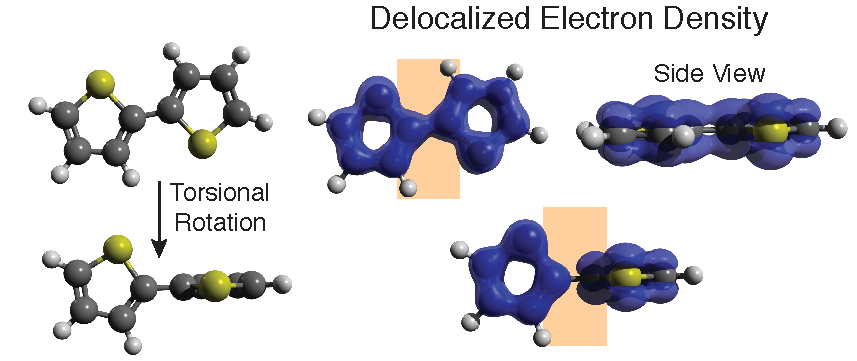
\includegraphics{figures/chap1_intro/figure_delocal_copy.pdf}
  \caption[Electron Density of Delocalized Bonds]{(Left) Two bithiophene torsional configurations, 180\textdegree \  (planar) on the top and 90\textdegree \ (non-planar) on the bottom. (Right) The electron density of delocalized bonds \cite{Szczepanik2017} isosurface plots (isovalue = 0.015). The isosurface of the non-planar configuration has a reduction in density between rings, which impacts its electronic properties. A side view of the planar configuration is included to display $\pi$-bonding pathways above and below the molecule.}
  \label{fig:eddb}
\end{figure*}

The atomic-scale structure of conjugated molecules and polymers plays a key role in determining carrier mobility and in turn electronic conductivity due to the geometric nature of $\pi$-bonding. In its completely planar undisturbed state, the $\pi$-bonding network in the electronic structure of the conjugated backbone provides an intramolecular conduction pathway for carriers. However, if a molecule or a chain is significantly torsioned (i.e. non-planar) the conduction pathway is disrupted. Figure \ref{fig:eddb} illustrates this point by comparing the delocalized electron density of a planar (top) and a non-planar (bottom) bithiophene torsional configuration. There is an electron deficient region between rings of the non-planar configuration, which represents a large energetic barrier that a carrier cannot overcome and hence represents a dead end for transport. These disruptions in conjugation are a product of polymer structure and limit carrier mobility and electronic conductivity.

As synthesized, conjugated polymer materials exhibit an intrinsic amount of structural disorder \cite{Noriega2013, Shen2016}, including non-planar configurations. This natural disorder introduces challenges for creating a micron-scale network of undisrupted pathways (i.e. no dead ends) for carrier transport. Although it is tempting to assume that more crystalline (i.e. ordered) materials would be more conductive, recent work indicates that less crystalline materials with undisrupted pathways are preferable \cite{Noriega2013, Son2016}. Part of the reason for this is that crystalline regions within the material are not guaranteed to align, creating many dead ends at the domain walls. Thus, a fundamental knowledge of structure, with predictive power at multiple length scales, is desirable to enable rationally designed engineering materials with undisrupted conjugation pathways. The central focus of this thesis is therefore to improve our understanding of amorphous (i.e. disordered) conjugated polymer structure at the electronic, atomic, and chain levels to inform design.

In Chapter 2 we concentrate on the topic of doped and excited polymer chain structure, utilizing a combination of quantum chemistry and statistical mechanics. Recent work by Son et al. and Noriega et al. demonstrate that carrier mobility in conjugated polymer materials is limited by the structure of the amorphous chains \cite{Noriega2013, Son2016}. Despite this fact, little is known about the impact doping or excitation have on the overall amorphous chain structure. To address this, we use a multiscale approach that captures relevant quantum mechanical effects with torsion potentials, which are then used to stochastically generate chain conformations. Using our model, we are able to quantify chain properties including planarity, and connect with a number of materials design approaches focused on improving electronic conductivity through structural modification.

Chapter 3 elucidates the underlying physics that determine planarity in a variety of conjugated molecules and polymers using quantum chemistry. We extend the results from Chapter 2, which clearly demonstrate that certain types of conjugated polymers exhibit a non-planar torsional minimum and identify the driving forces responsible for the non-planarity. We use aromaticity as a chemical descriptor to simplify the complex torsional energetics and guide us to the most relevant interactions for determining planar configurations. We find that hyperconjugation is a key interaction for noncovalent modification of aromaticity and control of planarity. Ultimately, the methods and the results can be used to inform molecular design.

An outlook is presented in Chapter 4 to discuss areas where research in Chapters 2 and 3 could be further developed.

\chapter{Structural Changes in Doped and Excited Conjugated Polymers}

first paper here
\chapter{Aromaticity as a Guide to Planarity in Conjugated Molecules and Polymers}

%%%%%%%%%%%%%%%%%%%%%%
\section{Introduction}

Organic semiconductors offer unique blends of physical and electronic properties along with the processability and fabrication potential of polymers and small molecules.\cite{Kuei2017, Swager2017} This combination opens up countless opportunities for new functional materials that can be tailored for specific applications.\cite{Mei2013, Muench2016, Someya2016, VanDeBurgt2018} One successful strategy for tuning molecular properties is adding pendent groups to the conjugated backbone; these ``noncovalent locks'' control molecular structure by inducing nonbonded interactions.\cite{Jackson2013, Cheng2016, Conboy2016, Huang2017}
The goal is to create structures that prefer coplanar torsional configurations that maximize electron delocalization across the molecule or polymer (i.e. conjugation), and as a result improve electronic properties such as carrier mobility.

While noncovalent locks have proven to be effective at creating planar structures, the exact nature of the interactions leading to planarity remain difficult to disentangle. A few reports have attempted to isolate and identify the fundamental interactions behind  noncovalent locking systems. For instance, Jackson et al. demonstrated that nontraditional hydrogen bonding (i.e. hydrogen bonding that involves less electronegative atoms such as C, S, and Cl) can play a predominant role in stabilizing planar configurations.\cite{Jackson2013} Nevertheless, many locking molecules such as 3,4-ethylenedioxythiophene (EDOT) and fluorinated thiophenes---which are utilized in state-of-the-art conjugated molecules and polymers\cite{Yum2014, Granstrom1995, Wijsboom2011, Gao2015, Gao2018, Jo2014, Li2015}---do not involve nontraditional hydrogen bonding. Conboy et al. confirmed the importance of heteroatom interactions in poly-EDOT (PEDOT) and similar molecules, but stated that a precise description of torsional energetics was unclear and speculated that electrostatics were responsible for the observed planarity.\cite{Conboy2016}

%It is difficult to disentangle which interactions are responsible for configurational preferences, however,
Aromaticity is a common chemical descriptor that can be used to simplify some of the underlying physics and provide novel insights into torsional energetics. A key objective of this communication is to highlight how the competition between aromaticity and conjugation\cite{Hernandez1994, Kertesz2005, Huang2017} influences planarity in organic electronic materials. We show that the introduction of popular noncovalent locks modifies aromaticity and drives structures towards planarity. Finally, we identity the specific hyperconjugation interaction that alters aromaticity and determines planarity.

%%%%%%%%%%%%%%%%%%%%%%%%%%%%%%%%
\section{Results and Discussion}

An illustrative example of the balance between ring aromaticity and conjugation is the torsion potential of bithiophene (BT) (Fig. 1). Dimers provide a computationally efficient and accurate representation of the torsion potential and trends in aromaticity observed in larger conjugated polymers (See SI)\cite{Dubay2012} and hence are used throughout this work. The aromaticity of individual rings is quantified using the multicenter bonding index (MCI),\cite{Giambiagi1990, Giambiagi2000} and the nucleus-independent chemical shift (NICS)\cite{Fallah-Bagher-Shaidaei2006, Chen2005} (see SI). We represent conjugation semi-quantitatively as the normalized relative bond length of the bridge C-C bond between rings; the rational being configurations with shorter bridge bonds are more conjugated.\cite{Daudey1980, Fernandez2006} Figure 1 (left side) clearly shows that the stabilizing effects of aromaticity and conjugation are in direct competition with one another. This agrees with a simple description based on atomic orbitals, where planar structures (0\textdegree \ cis and 180\textdegree \ trans) exhibit the most $p_z$-orbital overlap ($\pi$-bonding) and afford the most electron delocalization across the molecule. Whereas the torsioned structure at 90\textdegree \ will exhibit the least electron sharing between rings, and it possesses the highest ring aromaticity or electron delocalization within a ring. The non-planar global minimum (150\textdegree) in the torsion potential appears to be the balance between these two driving forces.

\begin{figure*}[hbt!]
    \centering
    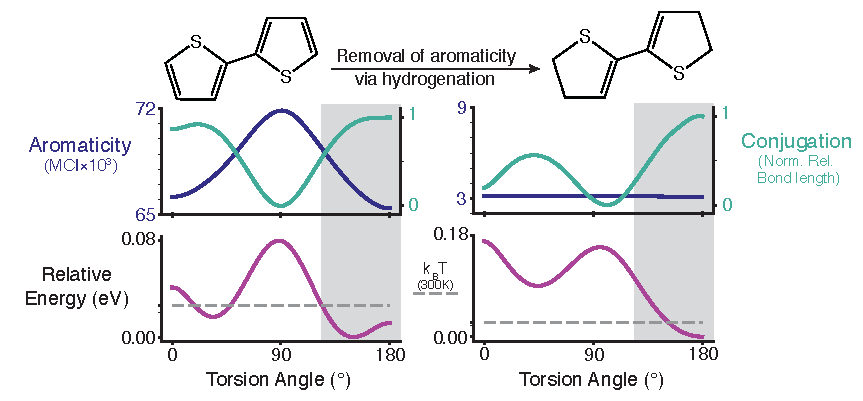
\includegraphics{figures/chap3/fig1_d2.pdf}
    \caption{Ring aromaticity, molecular conjugation, and relative energies are plotted as a function of torsion angle for bithiophene (BT) and hydrogenated bithiophene (hBT). Both BT and hBT structures are represented in the 180\textdegree \ (trans) configuration. Aromaticity and conjugation are directly opposed in BT and the balance between the two driving forces results in a non-planar torsional minimum around 150\textdegree. Hydrogenation of the terminal C-C double bonds essentially reduces aromaticity to zero, while preserving conjugation across the two rings. With aromaticity removed in hBT, torsional energetics mirror conjugation and there is a planar minimum at 180\textdegree. Aromaticity is defined as the multicenter bonding index (MCI$\times 10^3$) for one C-C-S-C-C thiophene ring. Only one ring is displayed because both BT and hBT are symmetric molecules. Conjugation is quantified as the normalized relative bridge C-C bond length. A value of 1 represents the shortest bond length and the highest conjugation, whereas 0 represents the longest bond and lowest amount of conjugation.}
    \label{fig:a_vs_c}
\end{figure*}

To test this hypothesis we removed aromaticity by hydrogenating the terminal C=C double bonds, leaving intact the conjugation across the rings (right side of Fig. 1). Once aromaticity was removed the torsional energetics essentially mirrored conjugation, and most importantly the global minimum in the torsion potential shifted to the planar 180\textdegree \ configuration. It is noteworthy that the inter-ring H$\cdots$S distance is reduced in hydrogenated bithiophene (hBT) (2.78\si{\angstrom} \ in the 180\textdegree \ configuration) compared to BT (2.93\si{\angstrom} \ in the 180\textdegree \ configuration), which reduces concern that the 150\textdegree \ torsional minimum in BT is due to steric repulsion between H$\cdots$S. This conclusion is supported with through-space calculations and noncovalent interaction (NCI) analysis\cite{Johnson2010, Contreras-Garcia2011} in the SI. Establishing aromaticity as a driving force in torsional energetics is fundamental for understanding structure; additionally, if aromaticity can be modified or controlled it may represent a design opportunity.

Having demonstrated the important role of aromaticity in directing torsion angles, we were motivated to explore the role of aromaticity in known planar systems with noncovalent locks. We discovered a number of reported noncovalent locks modify aromaticity. As observed in the top of Fig. 2 both  3,3'-difluorobithiophene (F2-BT) and bis-EDOT (BEDOT) exhibit a coplanar torsional minimum at 180\textdegree \ accompanied by an increase in aromaticity near 180\textdegree. As expected, conjugation is minimized at 90\textdegree \ and a maximized at 180\textdegree, it has been left out of Fig. 2 for clarity. For torsional energetics the magnitude of aromaticity is less important than the change in aromaticity. For example, if aromaticity is constant across all torsion angles there is no torsional driving force. As a result, we are interested in the change in aromaticity between 90-180\textdegree.

\begin{figure*}[hbt!]
    \centering
    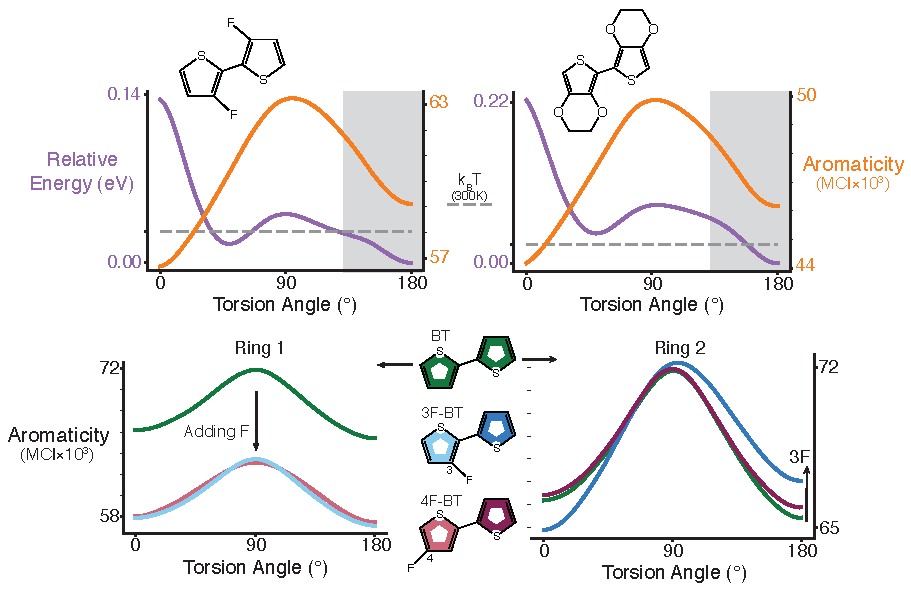
\includegraphics{figures/chap3/fig2_d7.pdf}
    \caption{(Top) Torsional relative energies and aromaticity are plotted for F2-BT and BEDOT. In both systems aromaticity is increased near 180\textdegree \ and this corresponds to an energetic minimum. (Bottom) Ring 1 and ring 2 aromaticities are plotted against torsion angles for BT, 3F-BT, and 4F-BT. Both rings are plotted because 3F-BT and 4F-BT molecules are no longer symmetric as is BT. For ring 1 the addition of F---regardless of the position---reduces the magnitude of aromaticity by a constant, but preserves the shape of the BT curve. The ring 2 curves are similar for 4F-BT and BT, however, ring 2 of 3F-BT deviates in shape and aromaticity is increased near 180\textdegree \ similar to the plots in the top of figure. }
    \label{fig2:a_mod}
\end{figure*}

To further investigate the modification of aromaticity we systematically added fluorine at different ring positions (bottom of Fig. 2). Notably, aromaticity increases near 180\textdegree \ in ring 2 (the ring without F added) of 3F-BT similarly to that of BEDOT and F2-BT in the top of Fig. 2. With only one added fluorine the aromaticity of both ring 1 and ring 2 need to be characterized because the molecule is no longer symmetric. When fluorine is added to ring 1---regardless of the position---it reduces the magnitude of aromaticity but preserves the shape of the curve (bottom left of Fig. 2), essentially reducing the underlying function by a constant. This is consistent with earlier reports that adding electron withdrawing substituents to an aromatic ring reduces the overall aromaticity.\cite{Krygowski2014} Naively, one might expect all thiophene rings without F added to be similar, and this is largely true for ring 2 of BT and 4F-BT but as mentioned ring 2 aromaticity is modified in 3F-BT. This result indicates that there is a noncovalent inter-ring interaction between F$\cdots$S causing the change in aromaticity.

Using Natural Bonding Orbital (NBO) analysis we identify the key interaction responsible for the modification of aromaticity and for stabilizing the planar 180\textdegree \ configuration (Fig. 3). Our through-space calculations for F$\cdots$S and O$\cdots$S indicate that both would be repulsive at the respective relaxed separation distance present in the 180\textdegree \ configuration of F2-BT and BEDOT (see SI). Thus, it is clear that some other interaction involving X$\cdots$S is stabilizing the steric effects in order for the 180\textdegree \ configuration to be energetically favorable. NBO perturbation analyses revealed a 3-center-2-electron interaction between a heteroatom lone pair and a C-S antibonding orbital ($\sigma^{*}_{C-S}$) pictured in the top of Fig. 3. Details on specific energies are provided in the SI. Similar interactions have been reported for the association of supramolecules.\cite{Cozzolino2005} Conboy et al. mentioned this type of interaction as a possible source of attraction in BEDOT-like molecules, but dismissed it due to a lack of bond length correlations across a series of related molecules.\cite{Conboy2016}

In order to confirm the importance of the 3-center-2-electron interaction we utilized the NBO deletion method\cite{NBO6}, which has been used previously to deconvolute torsional energetics.\cite{Pophristic2001} Because the NBO deletion method necessitates the use of restricted Hartree-Fock (RHF) we recalculated the torsion potentials with RHF to ensure qualitatively similar behavior to the higher level of theory ($\omega$B97x-D). Then using the RHF deletion method, we removed the C-S antibonding orbitals ($\sigma^{*}_{C-S}$) on both rings, which eliminates hyperconjugation. Remarkably, removing hyperconjugation altered the torsional energetics in both BEDOT and F2-BT such that the planar 180\textdegree \ configurations are no longer favorable (as shown in Figure 3), most likely due to the steric repulsion that exists. We characterize these as hyperconjugation interactions because they result in electron delocalization across the molecule and there is a history of hyperconjugation impacting torsional energetics.\cite{Pophristic2001, R.Rablen1999} This result provides strong evidence that hyperconjugation is the critical interaction responsible for the locking behavior in these molecules and polymers.

%%%%%%%%%%%%%%%%%%%%
\section{Conclusion}

Using a variety of computational techniques we have demonstrated that aromaticity is a useful descriptor to help understand the complex interactions which lead to the structure of conjugated molecules and polymers. In general, aromaticity is stabilizing and energetically favorable, and in extended conjugated molecules and polymers ring aromaticity prefers torsioned or non-planar configurations because it confines delocalized electrons within a ring instead of delocalizing them across the entire molecule or polymer. As such, aromaticity directly competes with conjugation, also known to be stabilizing and energetically favorable. BT is an ideal system to exemplify this competition, and ultimately we identify a balance between the two factors that results in a non-planar minimum energy configuration. Planarity and conjugation are vital for the electronic properties of conjugated materials so minimizing the driving force from aromaticity is industrially relevant. We find that aromaticity can indeed be beneficially modified through pendent group additions or noncovalent locks such as F2-BT and BEDOT. In both examples, a heteroatom interacts with an adjacent ring and increases its aromaticity at torsional angles near 180\textdegree \ where the atoms are the closest together. To probe the exact nature of this interaction we identified and removed hyperconjugation between a heteroatom (i.e. F and O) lone pair and the C-S antibonding orbital on the adjacent ring, concluding that hyperconjugation is responsible for the changes in aromaticity and for the resulting planarity or locking behavior. We anticipate that the structural insights and methods presented here are applicable to a wide range of conjugated molecules and polymers, and will open the door to new and unforeseen advances in our ability to design functional organic electronic materials.

%%%%%%%%%%%%%%%%%%%%%%%%%%%%%%%
\section{Computational Methods}

All quantum chemistry calculations were performed with Gaussian 16 unless otherwise noted.\cite{g16} The default level of theory was $\omega$B97x-D with the def2-TZVPP basis set.\cite{Chai2008, Weigend2005} The general procedure for calculating torsion potentials started with an unconstrained geometry relaxation followed by a frequency calculation to ensure no substantial imaginary frequencies existed. Then the relaxed geometry was rotated around the central C-C bond, fixing the C-C-C-C torsion every 10\textdegree \ for a constrained geometry optimization. An additional torsional constraint was used for hydrogenated calculations (See SI). MCI aromaticities were computed with the natural atomic orbital basis from NBO6 for all 5 member (C-C-S-C-C) rings at each torsional geometry using Multiwfn.\cite{Lu2012} NBO analysis was performed using NBO6.\cite{NBO6} All RHF and RHF NBO orbital deletions were done with Gaussian 09\cite{g09} and NBO6 again using the def2-TZVPP basis set. RHF NBO orbital deletions were single point calculations utilizing relaxed RHF geometries. Isosurface images were made with VMD,\cite{HUMP96} and all plotting utilized Matplotlib and cubic spline interpolation via SciPy.\cite{Jones}

\chapter{Outlook}

\section{Lessons Learned}

\begin{itemize}
  \item Do not eat directly before surfing
  \item Surf with a buddy
  \item Do not wax the bottom of the board

\end{itemize}

%\include{chap1}
%\include{chap2}

\printbibliography

\appendix
\chapter{Appendix for Aromaticity as a Guide to Planarity in Conjugated Molecules and Polymers}

\section{Different Length Polymer Chains}
\begin{figure}[hbt!]
    \centering
    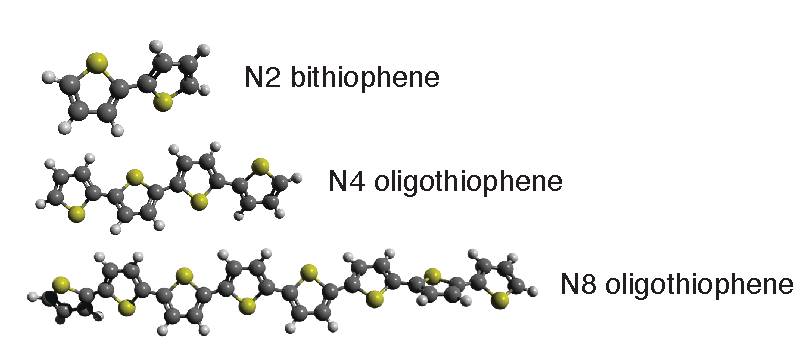
\includegraphics{figures/append_aroma/p_chains_graphic_copy.pdf}
    \caption{Different length oligomers of thiophene.}
    \label{fig:p_chains}
\end{figure}

\subsection{Comparison of Torsion Potentials}
\begin{figure}[hbt!]
    \centering
    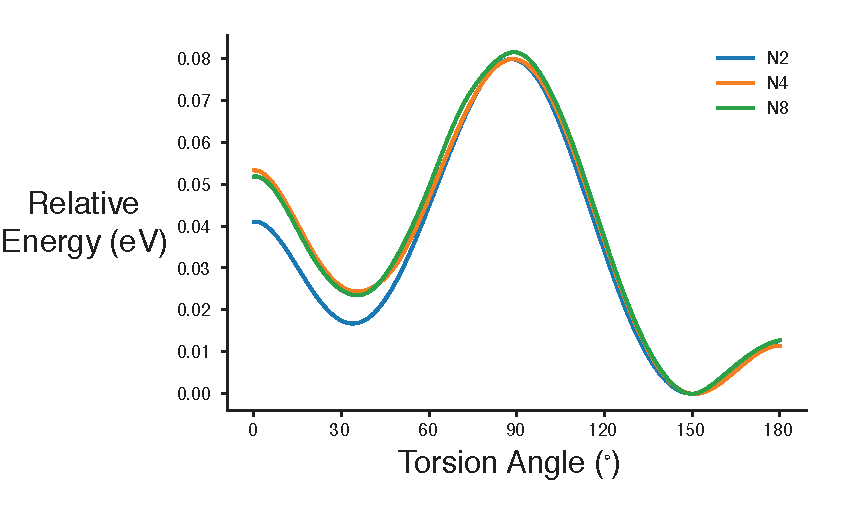
\includegraphics{figures/append_aroma/p_tor_compare_copy.pdf}
    \caption{The torsion potential of N2, N4, and N8 thiophene oligomers. All calculations were performed using the $\omega$B97x-D functional. The N2 torsion potential was calculated with the def2-TZVPP basis set, while N4 and N8 utilized the 6-31++G**\cite{Hehre1972} basis set to reduce to the computational cost. The deviation of N2 from both N4 and N8 between 0 and 50\textdegree \ is likely due to the different basis sets employed.}
    \label{fig:p_tor_compare}
\end{figure}

\clearpage
\subsection{Comparison of NICS Aromaticity}
\begin{figure}[hbt!]
    \centering
    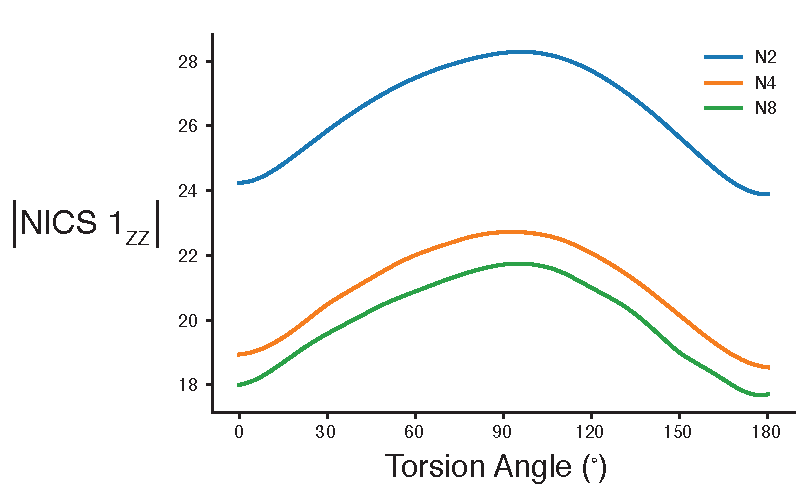
\includegraphics{figures/append_aroma/p_NICS_compare_copy.pdf}
    \caption{N2, N4, and N8 absolute NICS $1_{ZZ}$ values as a function of torsion angle. The magnitude of NICS values decrease with chain length, and we expected that the values will converge once a certain chain length is reached. While the magnitude decreases the overall trend as a function of torsion angle is consistent, which allows N2 to represent larger chains.}
    \label{fig:p_NICS_compare}
\end{figure}

\clearpage
\section{Comparision of MCI and NICS Aromaticity Values}

\subsection{BT}
\begin{figure}[hbt!]
    \centering
    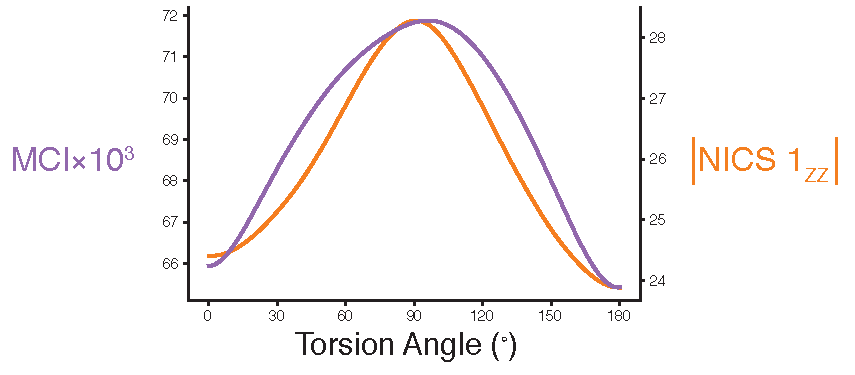
\includegraphics{figures/append_aroma/pt_aroma_compare_copy.pdf}
    \caption{Comparison of the aromaticity indexes MCI and NICS for BT.}
    \label{fig:pt_aroma_compare}
\end{figure}

\subsection{hBT}
\begin{figure}[hbt!]
    \centering
    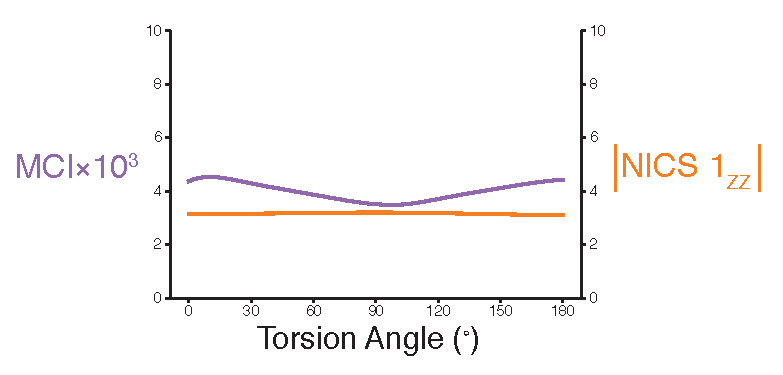
\includegraphics{figures/append_aroma/hpt_aroma_compare_copy.pdf}
    \caption{Comparison of the aromaticity indexes MCI and NICS for hBT.}
    \label{fig:hpt_aroma_compare}
\end{figure}

\clearpage
\subsection{F2-BT}
\begin{figure}[hbt!]
    \centering
    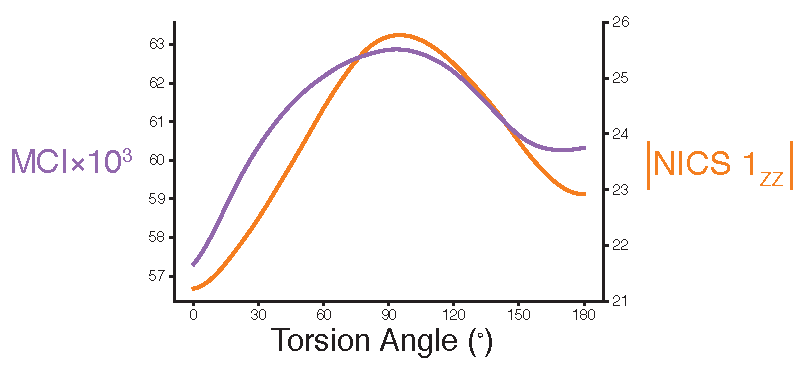
\includegraphics{figures/append_aroma/pt_f2_aroma_compare_copy.pdf}
    \caption{Comparison of the aromaticity indexes MCI and NICS for F2-BT.}
    \label{fig:pt_f2_aroma_compare}
\end{figure}


\subsection{BEDOT}
\begin{figure}[hbt!]
    \centering
    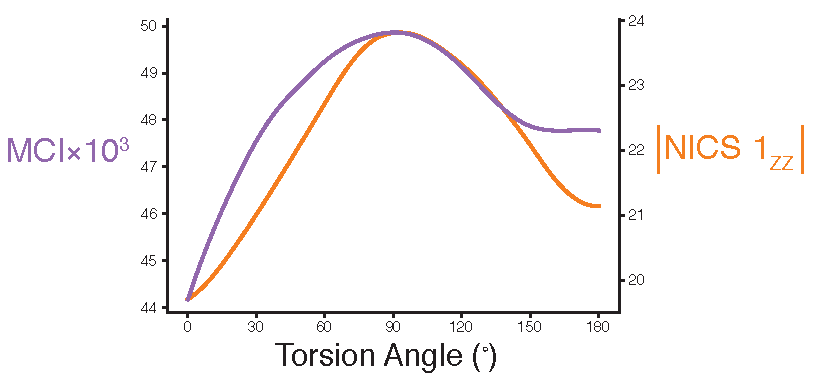
\includegraphics{figures/append_aroma/pedot_aroma_compare_copy.pdf}
    \caption{Comparison of the aromaticity indexes MCI and NICS for BEDOT.}
    \label{fig:pedot_aroma_compare}
\end{figure}

\clearpage
\section{Through-space Calculations}
\subsection{\texorpdfstring{H $\cdots$ S}{HS}}
\begin{figure}[hbt!]
    \centering
    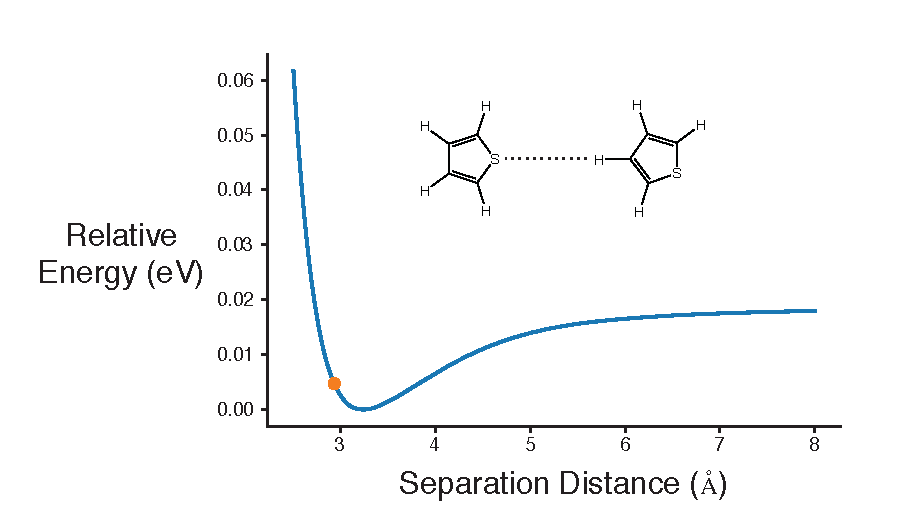
\includegraphics{figures/append_aroma/ts_t_t_copy.pdf}
    \caption{A potential energy scan of the interatomic separation distance between a hydrogen and a sulfur atom on thiophene molecules. The orange dot represents the relaxed H $\cdots$ S distance on a trans (180\textdegree) BT molecule. This indicates that the H $\cdots$ S through-space interaction is marginally repulsive in trans BT. It is noteworthy that the repulsive energy is small compared to the torsional barrier present at 180\textdegree \ in BT (a factor of $\sim$2.5), which in combination with the NCI analysis below demonstrate the minor role of sterics in determining planarity.}
    \label{fig:ts_t_t}
\end{figure}
\clearpage

\subsection{\texorpdfstring{H $\cdots$ S}{HSN} Noncovalent Interaction Analysis}
\begin{figure}[hbt!]
    \centering
    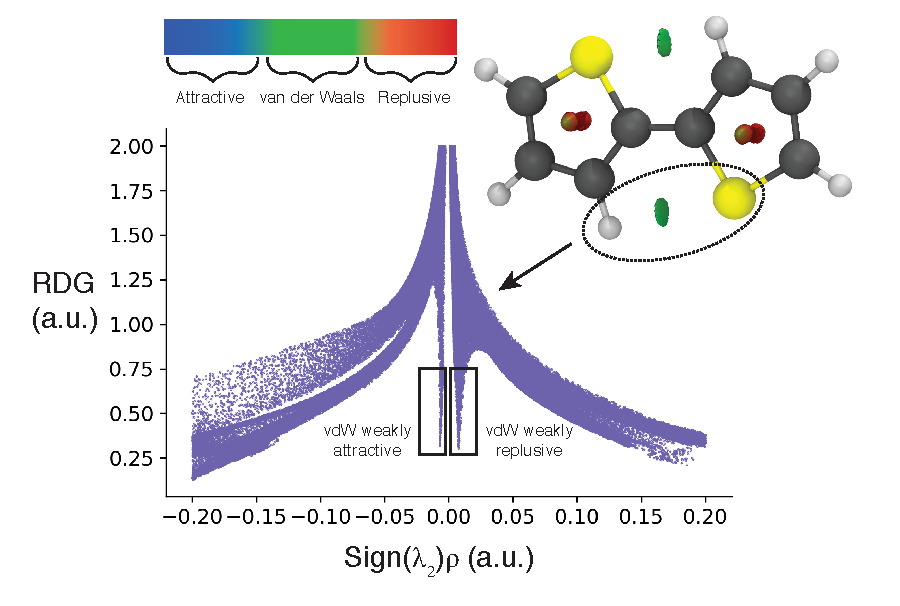
\includegraphics{figures/append_aroma/pt_nci_copy.pdf}
    \caption{The NCI analysis of BT including an NCI isosurface (right) and an s$(\rho$) plot (center), which displays the reduced density gradient (RDG) as a function of the sign of the electron-density Hessian matrix's second eiganvalue (sign$(\lambda_{2})$) times the electron-density ($\rho$). The isosurface plot on right shows a van der Waals interaction between H $\cdots$ S. The color gradient at the top gives a rough physical description of the color scheme used for the isosurface. When only the localized region around H $\cdots$ S is considered, by employing a radius cutoff, the s$(\rho$) plot is inconclusive exhibiting both weakly repulsive and weakly attractive interactions.}
    \label{fig:pt_nci}
\end{figure}
\clearpage

\subsection{\texorpdfstring{F $\cdots$ S}{FS}}
\begin{figure}[hbt!]
    \centering
    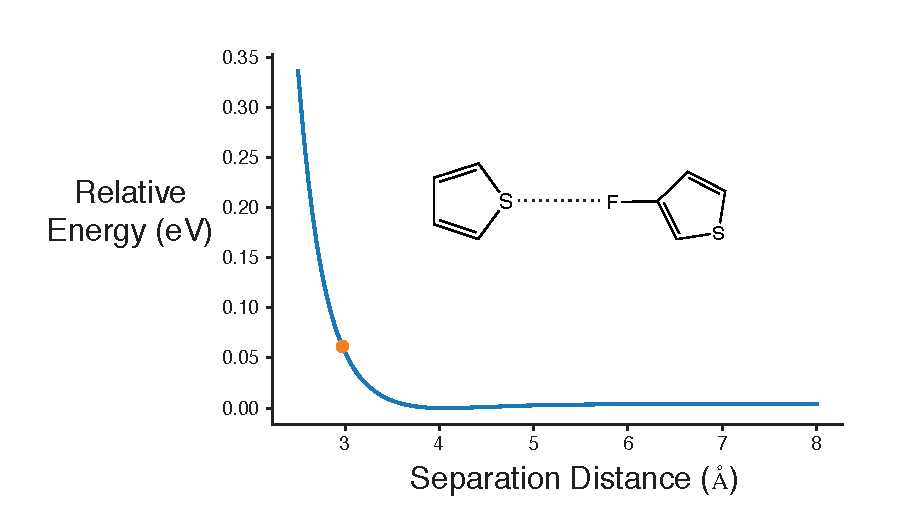
\includegraphics{figures/append_aroma/ts_t_t_f1_copy.pdf}
    \caption{A potential energy scan of the interatomic separation distance between a fluoride and a sulfur atom on a fluorinated thiophene and a thiophene molecule. The orange dot represents the relaxed F $\cdots$ S distance on a trans (180\textdegree) 3F-BT molecule. This indicates that the F $\cdots$ S through-space interaction is repulsive in trans 3F-BT.}
    \label{fig:ts_t_t_f1}
\end{figure}

\begin{figure}[hbt!]
    \centering
    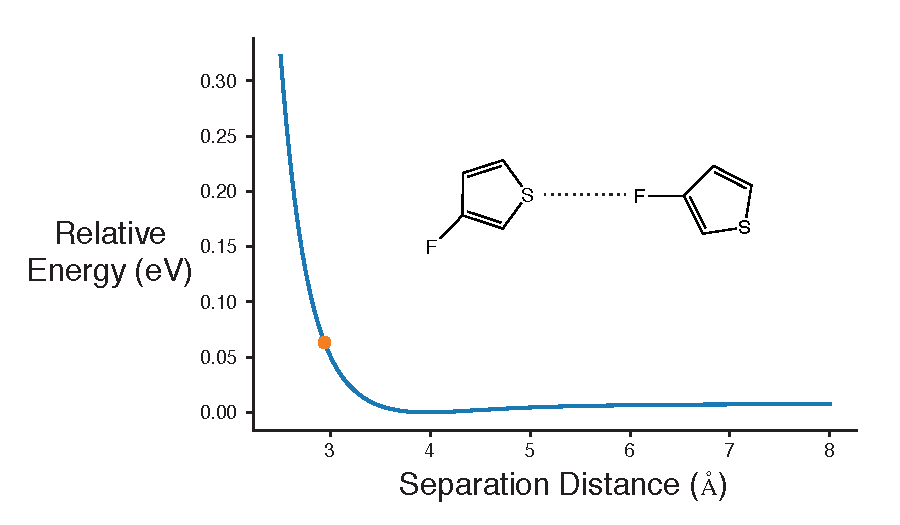
\includegraphics{figures/append_aroma/ts_2t_f1_copy.pdf}
    \caption{A potential energy scan of the interatomic separation distance between a fluoride and a sulfur atom on a fluorinated thiophene molecules. The orange dot represents the relaxed F $\cdots$ S distance on a trans (180\textdegree) F2-BT molecule. This indicates that the F $\cdots$ S through-space interaction is repulsive in trans F2-BT.}
    \label{fig:ts_2t_f1}
\end{figure}
\clearpage

\subsection{\texorpdfstring{F $\cdots$ S}{FSN} Noncovalent Interaction Analysis}
\begin{figure}[hbt!]
    \centering
    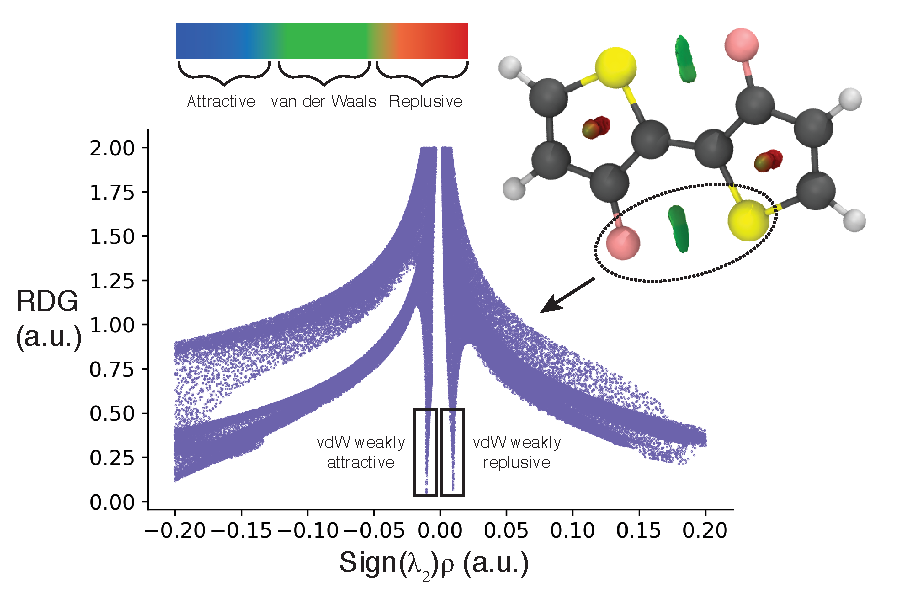
\includegraphics{figures/append_aroma/pt_f2_nciplot_copy.pdf}
    \caption{The NCI analysis of F2-BT including an NCI isosurface (right) and an s$(\rho$) plot (center), which displays the reduced density gradient (RDG) as a function of the sign of the electron-density Hessian matrix's second eiganvalue (sign$(\lambda_{2})$) times the electron-density ($\rho$). The isosurface plot on right shows a van der Waals interaction between H $\cdots$ S. The color gradient at the top gives a rough physical description of the color scheme used for the isosurface. When only the localized region around H $\cdots$ S is considered, by employing a radius cutoff, the s$(\rho$) plot is inconclusive exhibiting both weakly repulsive and weakly attractive interactions.}
    \label{fig:pt_f2_nci}
\end{figure}
\clearpage

\subsection{\texorpdfstring{O $\cdots$ S}{OS}}
\begin{figure}[hbt!]
    \centering
    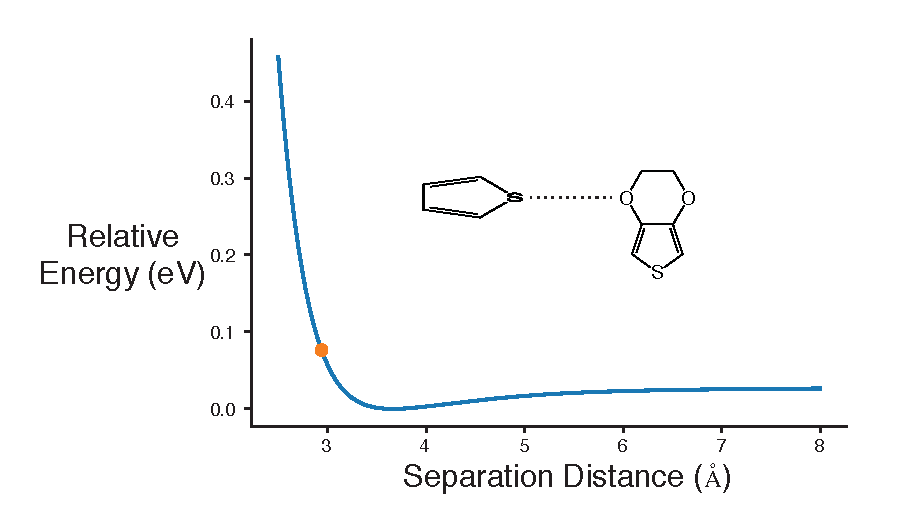
\includegraphics{figures/append_aroma/ts_t_edot_copy.pdf}
    \caption{A potential energy scan of the interatomic separation distance between a oxygen and a sulfur atom on an EDOT and thiophene molecule respectively. The thiophene molecule has been rotated such the ring is perpendicular to the EDOT ring, this is done to minimize secondary H $\cdots$ S interactions. The orange dot represents the relaxed O $\cdots$ S distance on a trans (180\textdegree) BEDOT molecule. This indicates that the O $\cdots$ S through-space interaction is repulsive in trans BEDOT.}
    \label{fig:ts_t_edot}
\end{figure}
\clearpage

\subsection{\texorpdfstring{O $\cdots$ S}{OSN} Noncovalent Interaction Analysis}
\begin{figure}[hbt!]
    \centering
    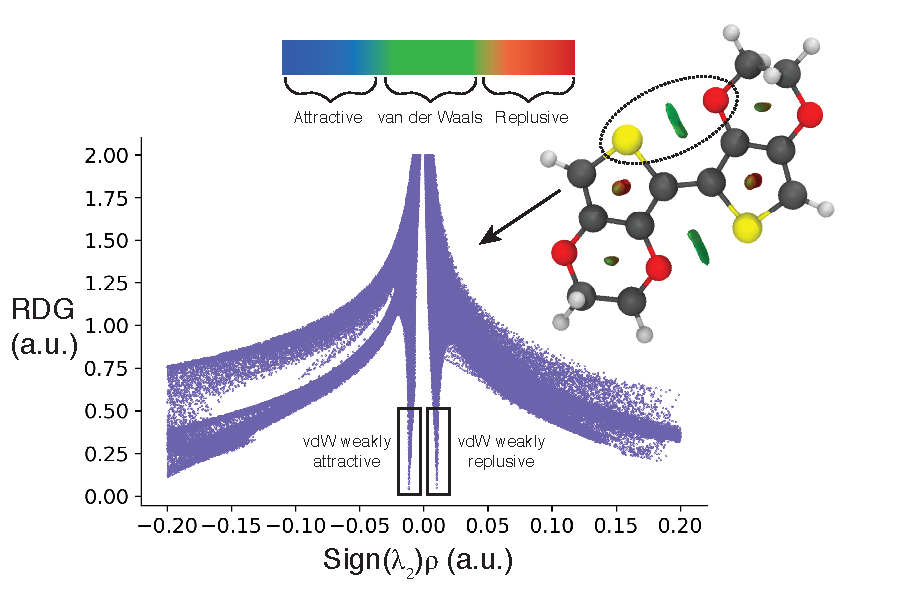
\includegraphics{figures/append_aroma/pedot_nciplot_copy.pdf}
    \caption{The NCI analysis of BEDOT including an NCI isosurface (right) and an s$(\rho$) plot (center), which displays the reduced density gradient (RDG) as a function of the sign of the electron-density Hessian matrix's second eiganvalue (sign$(\lambda_{2})$) times the electron-density ($\rho$). The isosurface plot on right shows a van der Waals interaction between H $\cdots$ S. The color gradient at the top gives a rough physical description of the color scheme used for the isosurface. When only the localized region around H $\cdots$ S is considered, by employing a radius cutoff, the s$(\rho$) plot is inconclusive exhibiting both weakly repulsive and weakly attractive interactions.}
    \label{fig:pedot_nci}
\end{figure}
\clearpage

% \chapter{More Monticello Candidates}

\end{document}
